%\everymath{\displaystyle}
\documentclass{beamer}
% \documentclass[handout]{beamer}

%\usepackage[pdftex]{color,graphicx}
\usepackage{amsmath,amssymb,amsfonts}

\mode<presentation>
{
  % \usetheme{Darmstadt}
  % \usetheme[hideothersubsections]{Hannover}
  % \usetheme[hideothersubsections]{Goettingen}
  \usetheme[hideothersubsections, right]{Berkeley}

  \usecolortheme{seahorse}
  % \usecolortheme{dolphin}
  \usecolortheme{rose}
  % \usecolortheme{orchid}

  \useinnertheme[shadow]{rounded}

  \setbeamercovered{transparent}
  % or whatever (possibly just delete it)
}

\mode<handout>{
  \setbeamercolor{background canvas}{bg=black!5}
  \usepackage{pgfpages}
  \pgfpagesuselayout{4 on 1}[a4paper,border shrink=5mm, landscape]
}

\usepackage[brazilian]{babel}
% or whatever

% \usepackage[latin1]{inputenc}
\usepackage[utf8]{inputenc}
% or whatever

\usepackage{times}
%\usepackage[T1]{fontenc}
% Or whatever. Note that the encoding and the font should match. If T1
% does not look nice, try deleting the line with the fontenc.


\title%[] % (optional, use only with long paper titles)
{Probabilidades I}

\subtitle
{Probabilidades básicas} % (optional)

\author%[] % (optional, use only with lots of authors)
{Felipe Figueiredo}% \and S.~Another\inst{2}}
% - Use the \inst{?} command only if the authors have different
%   affiliation.

\institute[INTO] % (optional, but mostly needed)
{Instituto Nacional de Traumatologia e Ortopedia}
  % \inst{1}%
  % Department of Computer Science\\
  % University of Somewhere
  % \and
  % \inst{2}%
  % Department of Theoretical Philosophy\\
  % University of Elsewhere}
% - Use the \inst command only if there are several affiliations.
% - Keep it simple, no one is interested in your street address.

\date%[Março de 2015] % (optional)
{}

% \subject{Talks}
% This is only inserted into the PDF information catalog. Can be left
% out. 



% If you have a file called "university-logo-filename.xxx", where xxx
% is a graphic format that can be processed by latex or pdflatex,
% resp., then you can add a logo as follows:

\pgfdeclareimage[height=1.6cm]{university-logo}{../logo}
\logo{\pgfuseimage{university-logo}}



% Delete this, if you do not want the table of contents to pop up at
% the beginning of each subsection:
\AtBeginSubsection[]
%\AtBeginSection[]
{
  \begin{frame}<beamer>{Sumário}
    \tableofcontents[currentsection,currentsubsection]
  \end{frame}
}


% If you wish to uncover everything in a step-wise fashion, uncomment
% the following command: 

\beamerdefaultoverlayspecification{<+->}


\begin{document}

\begin{frame}
  \titlepage
\end{frame}

\begin{frame}{Sumário}
  \tableofcontents
  % You might wish to add the option [pausesections]
\end{frame}


%% Template
% \section{}

% \subsection{}

% \begin{frame}{}
%   \begin{itemize}
%   \item 
%   \end{itemize}
% \end{frame}

% \begin{frame}
%   \begin{columns}
%     \begin{column}{5cm}
%     \end{column}
%     \begin{column}{5cm}
%     \end{column}
%   \end{columns}
% \end{frame}

% \begin{frame}{}
%   \includegraphics[height=0.4\textheight]{file1}
%   \includegraphics[height=0.4\textheight]{file2}
%   \includegraphics[height=0.4\textheight]{file3}
%   \begin{figure}
%     \caption{}
%   \end{figure}
% \end{frame}

% \section{Probabilidades}

% \begin{frame}{}
%   \begin{itemize}
%   \item 
%   \end{itemize}
% \end{frame}

\section{Definições}

\begin{frame}{Definições}
  \begin{definition}
    {\bf Experimento aleatório} é um experimento no qual se conhece os
    resultados possíveis, mas não se pode saber qual ocorrerá.
  \end{definition}

  \begin{itemize}
  \item Caso repetido em condições idênticas, o resultado geralmente é
    diferente.
  \item Formulam-se esses problemas de acordo com alguns conjuntos
    típicos.
  \end{itemize}

\end{frame}

\begin{frame}{Definições}
  \begin{definition}
    {\bf Espaço amostral} (S) é o conjunto de todos os resultados
    possíveis no problema.
  \end{definition}
  \begin{definition}
    {\bf Evento} (E) é o conjunto dos resultados favoráveis no
    problema. Qualquer subconjunto do espaço amostral.
  \end{definition}
  \begin{itemize}
  \item De quantas maneiras um evento pode ocorrer?
  \item Contar a quantidade (tamanho do conjunto) e dividir pela
    quantidade total de possibilidades
  \end{itemize}
\end{frame}

\begin{frame}{Definições}
  \begin{definition}
    A {\bf probabilidade} P(E) do evento E é a razão entre o número de
    elementos do evento E e do espaço amostral S. Entende-se pela
    \alert{frequência} de ocorrência do evento E.
    \begin{displaymath}
      P(E) = \frac{\#E}{\#S}
    \end{displaymath}
  \end{definition}
  \begin{example}
    Para se determinar a probabilidade de uma pessoa estar infectada
    com o Dengue em uma amostra pode-se considerar a frequência
    relativa do número de infectados em relação ao total da amostra.
  \end{example}
\end{frame}

% \subsection{Propriedades}

\begin{frame}{Propriedades das probabilidades}
  \begin{itemize}
  \item Evento impossível: $P(\emptyset) = 0$
  \item Evento certo: $P(S) = 1$
  \item $0 \le P(E) <= 1 (=100\%)$
  \end{itemize}
\end{frame}


% \begin{frame}{Propriedades das probabilidades}

%   \begin{example}
    
%   \end{example}

% \end{frame}



\begin{frame}%{Definições}
  \begin{example}
Probabilidade de observar cara em uma moeda:
\begin{displaymath}
  P(\text{cara}) = \frac{1}{2}
\end{displaymath}
  \end{example}

  \begin{example}
Probabilidade de observar um número par num dado
    \begin{displaymath}
      P( \text{par} ) = \frac{3}{6} = \frac{1}{2}
    \end{displaymath}
  \end{example}

  \begin{example}
Probabilidade de sortear um ás no baralho
    \begin{displaymath}
      P( A ) = \frac{4}{52} = \frac{1}{13}
    \end{displaymath}
  \end{example}

\end{frame}

\begin{frame}%{Definições}
  \begin{example}<1-> 
    Um casal tem três filhos. Qual é a probabilidade de que duas das
    três crianças sejam meninos?
    \bigskip
    \begin{columns}
      \begin{column}{5cm}
        \begin{tabular}{c}
          menino-menina-menina\\
          \alert<3->{menino-menina-menino}\\
          \alert<3->{menino-menino-menina}\\
          menino-menino-menino\\
          menina-menino-menina\\
          \alert<3->{menina-menino-menino}\\
          menina-menina-menina\\
          menina-menina-menino\\
        \end{tabular}
      \end{column}
      \uncover<4->{\begin{column}{5cm}
        \begin{itemize}
        \item<4-> 3 casos no evento
        \item<4-> \alert{M}F\alert{M}, \alert{MM}F, F\alert{MM}
        \item<4-> 8 possibilidades (\alert{total})
        \item<5-> $P( \text{dois meninos}) = \frac{3}{8}$
        \end{itemize}
      \end{column} }
    \end{columns}
  \end{example}
\end{frame}

\begin{frame}{Exercícios}
  \begin{block}{Exercício}
    De acordo com o problema anterior, qual é a probabilidade de
    \begin{enumerate}
    \item Exatamente uma menina?
    \item Exatamente duas meninas?
    \item Três meninas?
    \end{enumerate}
  \end{block}
  \begin{block}{Solução}
    \begin{enumerate}
    \item $\frac{3}{8}$ (MM\alert{F}, M\alert{F}M, \alert{F}MM)
    \item $\frac{3}{8}$ (M\alert{FF}, \alert{F}M\alert{F}, \alert{FF}M)
    \item $\frac{1}{8}$ (FFF)
    \end{enumerate}
  \end{block}
\end{frame}

\begin{frame}{Definições}
  \begin{definition}
    O {\bf complemento} $\bar{E}$ (ou $E^c$) de um evento E consiste
    em todas as possibilidades em que o evento E \alert{não} ocorre.
  \end{definition}
  \begin{definition}
    {\bf Probabilidade complementar} $P(\bar{E})$ (ou $P(E^c)$) de um
    evento E é a probabilidade do evento E \alert{não} ocorrer.
    \begin{displaymath}
      P(\bar{E}) = 1 - P(E)
    \end{displaymath}
  \end{definition}
\end{frame}

\begin{frame}{Exercícios}
  \begin{block}{Exercício}
    Qual é a probabilidade de se observar um número ímpar no dado?
  \end{block}
  \begin{block}{Solução}
    \begin{displaymath}
      P(\text{ímpar}) = 1-P(\text{par}) = 1-\frac{1}{2} = \frac{1}{2}
    \end{displaymath}
  \end{block}
  \begin{block}{Exercício}
    Qual é a probabilidade de se sortear uma carta no baralho que não
    seja um ás?
  \end{block}
  \begin{block}{Solução}
    \begin{displaymath}
      P(\bar{A})   = 1 - P(A) = 1- \frac{1}{13} = \frac{12}{13}
    \end{displaymath}
  \end{block}
\end{frame}

\begin{frame}{Até aqui...}
  \begin{itemize}
  \item Até aqui vimos a probabilidade de \alert{um} evento E.
  \item Normalmente precisamos cruzar informações de \alert{vários} eventos.
  \item Nesses casos, precisamos de dois conceitos fundamentais para o futuro \ldots
  \end{itemize}
\end{frame}

\section{Regra da soma}

% \subsection{Exclusividade mútua}

\begin{frame}{Um novo tipo de pergunta (1)}
  \begin{example}
    \begin{itemize}
    \item Considere 4 tipos de sintomas (S) e dois estágios de doença:
      terminal (T) e não terminal (N).

    \item Qual é a probabilidade de um paciente ter o sintoma 3
      \alert{{\bf ou}} ser um paciente terminal?

    \end{itemize}
  \end{example}

  Para construirmos a resolução deste tipo de pergunta, precisamos
  entender o que são eventos mutuamente exclusivos.
\end{frame}

\begin{frame}{Eventos compostos}
  \begin{example}
    Quantas ervilhas têm caule verde \alert{ou} flor roxa?
  \end{example}
  \begin{figure}
    \centering
    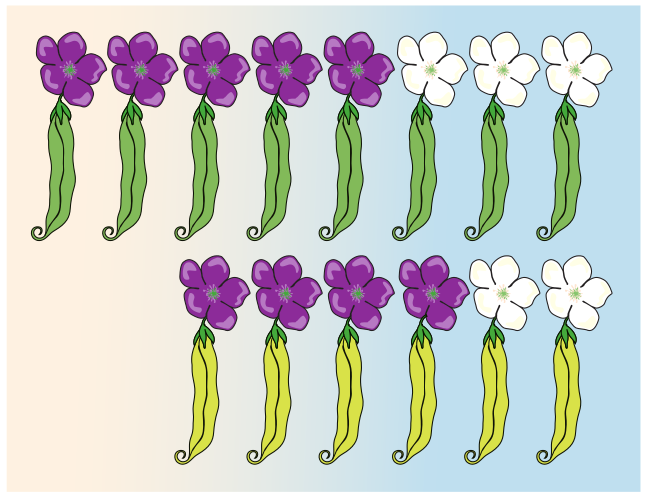
\includegraphics[height=0.6\textheight]{Prob_I/ervilhas-genetica}
    \caption{Fonte: Triola, 2004.}
  \end{figure}
\end{frame}

% \subsection{Regra da Soma}

\begin{frame}{Regra da Soma}
  \begin{definition}
    P (A \text{ ou } B) = P(A) + P(B) - P(A \text{ e } B)
  \end{definition}
  \begin{block}{Interpretação}
    P (A \text{ ou } B) = P(A ocorre ou B ocorre ou ambos ocorrem)
  \end{block}
  \begin{itemize}
  \item Atenção: não podemos contabilizar o evento P(A e B) duas
    vezes.
  \end{itemize}
\end{frame}

\begin{frame}{Eventos mutuamente exclusivos}
  \begin{itemize}
  \item Não podem ocorrer simultaneamente
  \item Eventos (conjuntos) disjuntos
  \end{itemize}
  \begin{figure}
    \centering
    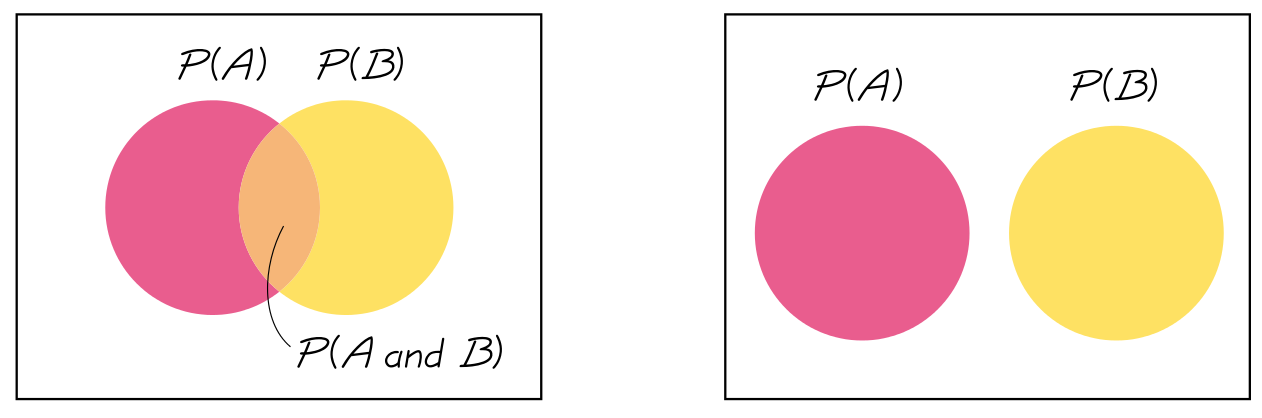
\includegraphics[height=0.4\textheight]{Prob_I/venn}
    \caption{Fonte: Triola, 2004.}
  \end{figure}
\end{frame}

\begin{frame}{Eventos mutuamente exclusivos}
  \alert{Não são} mutuamente exclusivos
  \begin{example}
    \begin{tabular}{l}
      A = Escolher estudante\\
      B = Escolher mulher\\
    \end{tabular}
  \end{example}
  \begin{example}
    \begin{tabular}{l}
      A = Escolher mulher\\
      B = Escolher tipo sanguíneo O+\\
    \end{tabular}
  \end{example}
  \begin{example}
    \begin{tabular}{l}
      A = Escolher homem\\
      B = Escolher olhos castanhos\\
    \end{tabular}
  \end{example}
\end{frame}

\begin{frame}{Eventos mutuamente exclusivos}
  \alert{São} mutuamente exclusivos
  \begin{example}
    Sortear uma carta no baralho
    \begin{tabular}{l}
      A = Observar um valete\\
      B = Observar um rei\\
    \end{tabular}
  \end{example}
  \begin{example}
    \begin{tabular}{l}
      A = Estar grávida\\
      B = Não estar grávida\\
    \end{tabular}
  \end{example}
  \begin{example}
    \begin{tabular}{l}
      A = Tipo sanguíneo A\\
      B = Tipo sanguíneo B\\
    \end{tabular}
  \end{example}
\end{frame}

\begin{frame}{Eventos mutuamente exclusivos}
  \begin{itemize}
  \item Se A e B são mutuamente exclusivos, P(A \text{ e } B)=0
  \item Nesse caso, P(A \text{ ou } B) = P(A)+P(B)
  \end{itemize}
\end{frame}

\begin{frame}{Exercícios}
  \begin{block}{Exercício}
    Você sorteia uma carta em um baralho comum. Qual é a probabilidade
    de se observar um valete ou um rei?
  \end{block}
  \begin{block}{Solução}
    \begin{displaymath}
      P(J \text{ ou } K) = \frac{4}{52} + \frac{4}{52} = \frac{8}{52} = \frac{2}{13}
    \end{displaymath}
  \end{block}
\end{frame}

\begin{frame}{Pergunta 1 (lembra?)}
  \begin{example}
    \begin{columns}
      \begin{column}{5cm}<1->
        4 sintomas e estágios terminal e não terminal (T/N).

        \smallskip
        Qual é a probabilidade de um paciente ter náusea {\bf ou} ser terminal?
      \end{column}
      \begin{column}{5cm}<1->
        \begin{tabular}{ccc|c}
          Sintoma & T & N & total\\
          \hline
          febre & 3 & 4 & 7\\
          diarréia & 5 & 0 & 5\\
          náusea & \alert<9>{4} & 8 & \alert<5>{12}\\
          vômito & 0 & 12 & 12\\
          \hline
          total & \alert<6>{12} & 24 & \alert<5,6,9>{36}\\
        \end{tabular}
      \end{column}
    \end{columns}
  \end{example}
  \begin{block}{Solução}
    \begin{columns}
      \begin{column}{4cm}<5->
        \alert<5>{A = náusea}

        \alert<6>{B = terminal}

        \smallskip
        \only<7->{P(A) = $\frac{12}{36} = \frac{1}{3}$}

        \only<7->{P(B) = $\frac{12}{36} = \frac{1}{3}$}
      \end{column}
      \begin{column}{6cm}<8->
        \begin{itemize}
        \item<8-> P(A) = $\frac{1}{3}$, P(B) = $\frac{1}{3}$
        \item<9-> P(A e B) = $\alert<9>{\frac{4}{36}} = \frac{1}{9}$
        \item<10-> P(A ou B) = $\frac{1}{3} + \frac{1}{3} - \frac{1}{9} = \frac{5}{9}$
        \end{itemize}
      \end{column}
    \end{columns}
  \end{block}
\end{frame}

\begin{frame}{Exercícios}
  \begin{block}{Exercício}
    \begin{tabular}{ccccc|c}
      & O & A & B & AB & total\\
      \hline
      Rh+ & 156 & 139 & 37 & 12 & 344\\
      Rh- & 28 & 25 & 8 & 4 & 65\\
      \hline
      total & 184 & 164 & 45 & 16 & 409\\
    \end{tabular}
    \begin{enumerate}
    \item<1-> Quantas pessoas tem sangue O ou A?
    \item<1-> Quantas pessoas tem sangue B ou Rh-?
    \end{enumerate}
  \end{block}
  \begin{block}{Solução}
    \begin{enumerate}
    \item P(O ou A) = $\frac{184}{409}$ + $\frac{164}{409}$ =
      $\frac{348}{409} \approx 0.85$
    \item P(B ou Rh-) = $\frac{45}{409}$+ $\frac{65}{409}$ -
      $\frac{8}{409}$ = $\frac{102}{409} \approx 0.25$
    \end{enumerate}
  \end{block}
\end{frame}

\section{Regra da Multiplicação}

% \subsection{Eventos Dependentes}

\begin{frame}{Um novo tipo de pergunta (2)}
  \begin{example}
    \begin{itemize}
    \item Pesquisadores querem cruzar duas informações \ldots
    \item \ldots contaram crianças que tem um certo gene G e aferiram seus
      QIs.
    \item Qual é a probalidade de uma criança possuir QI elevado
      \alert{{\bf e}} ter o gene G?
    \end{itemize}
  \end{example}

  Para construirmos a resolução deste tipo de pergunta, precisamos entender o que são eventos independentes.
\end{frame}

\begin{frame}{Regra da Multiplicação}
  \begin{itemize}
  \item Como determinar a probabilidade de dois eventos A e B
    ocorrerem simultaneamente?
  \item Para calcular isso, precisamos primeiro determinar se eles são
    \alert{dependentes} ou \alert{independentes}.
  \item Assim, podemos aplicar a Regra da Multiplicação.
  \end{itemize}
\end{frame}

\begin{frame}{Eventos dependentes}
  Se você retirar duas ervilhas \alert{sem reposição} dessa amostra,
  qual a probabilidade de de a primeira ter caule verde, e a segunda
  ter caule amarelo?
  \begin{figure}
    \centering
    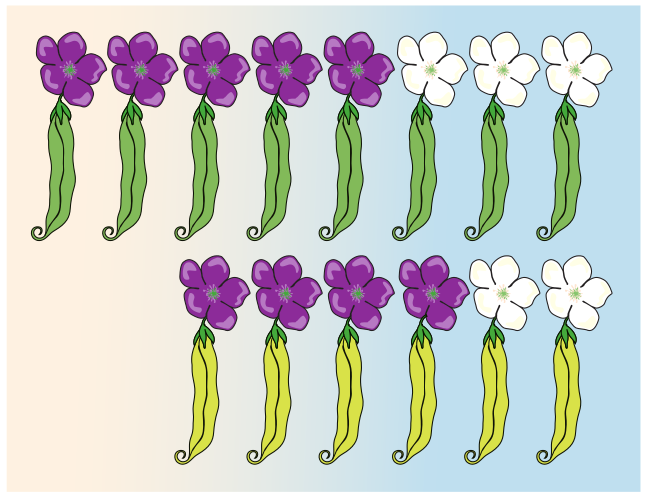
\includegraphics[height=0.5\textheight]{Prob_I/ervilhas-genetica}
    \caption{Fonte: Triola, 2004.}
  \end{figure}
\end{frame}

\begin{frame}{Eventos dependentes}
  Se você retirar duas ervilhas \alert{sem reposição} dessa amostra,
  qual é a probabilidade de a primeira ter caule verde, e a segunda
  ter caule amarelo?  
\bigskip
\bigskip
\bigskip
  \begin{block}{Solução}
    Primeira ervilha:
    \begin{displaymath}
      P(\text{verde}) = \frac{8}{14}
    \end{displaymath}
    Segunda ervilha:
    \begin{displaymath}
      P(\text{amarelo}) = \frac{6}{13}
    \end{displaymath}
  \end{block}
\end{frame}

\begin{frame}{Eventos dependentes}
  \begin{itemize}
  \item Observe que o segundo evento foi influenciado pelo primeiro!
  \item Isso modifica a probabilidade do segundo ocorrer
    \alert{depois} do primeiro.
  \item Lê-se: probabilidade do segundo ocorrer \alert{dado} que o
    primeiro ocorreu.
  \end{itemize}
\end{frame}

% \subsection{Probabilidade Condicional}
\begin{frame}{Probabilidade condicional}
  \begin{definition}
    \begin{displaymath}
      P(B|A) = \frac{P(A \text{ e } B)}{P(A)}, \text{ se } P(A)>0
    \end{displaymath}
  \end{definition}
  \begin{block}{Interpretação}
    $P(B|A)$ = Probabilidade de B ocorrer, \alert{dado que} A ocorreu.
  \end{block}
  \begin{itemize}
  \item Manipulando a fórmula, temos que $P(A \text{ e } B) =
    P(A)P(B|A)$ (regra da multiplicação)
  \end{itemize}
\end{frame}

\begin{frame}{Eventos Dependentes}
  \begin{example}
    Pesquisadores contaram crianças que tem um certo gene G e seus QIs

    \begin{tabular}{ccc|c}
      QI & possui o gene & não possui o gene & total\\
      elevado & 33 & 19 & 52\\
      normal & 39 & 11 & 50\\
      \hline
      total & 72 & 30 & 102\\
    \end{tabular}

    Qual é a probabilidade de uma criança ter QI elevado, dado que ela
    possui o gene G?
  \end{example}
  \begin{block}{Solução}
    \begin{displaymath}
      P(\text{QI elevado}| G) = \frac{33}{72}
    \end{displaymath}
  \end{block}
\end{frame}

% \begin{frame}{Eventos dependentes}
% \end{frame}

\begin{frame}{Exercício}
  \begin{block}{Exercício}
    \begin{tabular}{ccc|c}
      QI & possui o gene & não possui o gene & total\\
      elevado & 33 & 19 & 52\\
      normal & 39 & 11 & 50\\
      \hline
      total & 72 & 30 & 102\\
    \end{tabular}
    \begin{enumerate}
    \item Qual é a probabilidade de uma criança não ter o gene?
    \item Qual é a probabilidade de uma criança não ter o gene, dado
      que ela tem o QI normal?
    \end{enumerate}
  \end{block}
\end{frame}

\begin{frame}{Exercício}
  \begin{block}{Solução}
  \begin{tabular}{ccc|c}
    QI & possui o gene & não possui o gene & total\\
    elevado & 33 & 19 & 52\\
    normal & 39 & 11 & 50\\
    \hline
    total & 72 & 30 & 102\\
  \end{tabular}
    \begin{enumerate}
    \item $P(\bar{G}) = \frac{30}{102}$
    \item $P(\bar{G}|N) = P(N)P(\bar{G} \text{ e } N)$
      \begin{displaymath}
        P(N) = \frac{50}{102}
      \end{displaymath}
      \begin{displaymath}
        P(\bar{G} \text{ e } N) = \frac{11}{102}
      \end{displaymath}
      \begin{displaymath}
        P(\bar{G}|N) = \frac{11}{50}
      \end{displaymath}
    \end{enumerate}
  \end{block}
\end{frame}

% \section{Independência}

\begin{frame}{Eventos Independentes}
  \begin{definition}
    \begin{displaymath}
      P(B|A) = P(B)
    \end{displaymath}
  \end{definition}
  \begin{block}{Interpretação}
    Se dois eventos A e B são independentes a ocorrência de um não
    afeta a ocorrência do outro.
  \end{block}
  % \begin{itemize}
  % \item Se dois eventos são independentes, então 
  % \end{itemize}
\end{frame}


\begin{frame}{Regra da Multiplicação}
  \begin{itemize}
  \item No caso geral, a regra da multiplicação segue a fórmula $P(B \text{ e } A) = P(A)P(B|A)$
  \item Mas se A e B são independentes, então $P(B|A) = P(B)$
  \item Nesse caso, $P(B \text{ e } A) = P(A)P(B)$
  \end{itemize}
\end{frame}

\begin{frame}{Exercícios}
  \begin{block}{Exercício}
    Considere a tabela que relaciona resultados de teste de gravidez
    com o desfecho de estar ou não grávida
    \begin{tabular}{ccc|c}
      & teste positivo & teste negativo & total\\
      grávida & 80 & 5 & 85\\
      não grávida & 3 & 11 & 14\\
      \hline
      total & 83 & 16 & 99\\
    \end{tabular}
    \begin{enumerate}
    \item Determine a probabilidade de a mulher testar positivo, dado
      que ela está grávida
    \item Determine a probabilidade de a mulher estar grávida, dado
      que ela testou positivo
    \end{enumerate}
  \end{block}
\end{frame}

\begin{frame}{Exercícios}
  \begin{block}{Solução}
    \begin{tabular}{ccc|c}
      & teste positivo & teste negativo & total\\
      grávida & 80 & 5 & 85\\
      não grávida & 3 & 11 & 14\\
      \hline
      total & 83 & 16 & 99\\
    \end{tabular}
    \begin{enumerate}
    \item P(positivo$|$grávida) = 
      \begin{displaymath}
        \frac{\frac{80}{99}}{\frac{85}{99}} = \frac{80}{85} \approx 0.941
      \end{displaymath}
      Alternativamente, apenas consultando a tabela:
      P(positivo$|$grávida) = $\frac{80}{85} \approx 0.941$

    \item P(grávida$|$positivo) = $\frac{80}{83} \approx 0.964$
    \end{enumerate}
  \end{block}
\end{frame}

\section{Resumo}

\begin{frame}{Resumo}
  \begin{itemize}
  \item Para se determinar a probabilidade de um evento simples, basta
    considerar a frequência com que ele ocorre
  \item Para se calcular a probabilidade de um evento composto de um
    evento A \alert{ou} um evento B usamos a regra da soma
  \item Para se calcular a probabilidade de um evento composto de um
    evento A \alert{e} um evento B (simultaneamente) usamos a regra da
    multiplicação
  \item Em geral $P(A|B) \neq P(B|A)$
  \end{itemize}
  
\end{frame}

\end{document}

